\section{Software Interface}
\label{sec:software}

In FlashBoost, we aim to provide a set of software interfaces that support the
execution of any existing application as well as modified applications that
leverage the in-store processors in the system. Furthermore, software layers in
FlashBoost must perform flash management functions since we chose to expose a
raw flash interface in hardware for higher efficiency (previous discussed in
Section~\ref{sec:flashInterface}). The software architecture is shown in
Figure~\ref{fig:filesystem}.  Three interfaces are supplied to the user
application: (i) a file system interface, (ii) block device driver interface
and (iii) an accelerator interface. 

%The primary design goal of the FlashBoost file system layer is to provide an
%easy-to-use interface between user-level applications and hardware accelerators
%in the storage device, by hiding many of the complex physical properties of
%flash storage. Since NAND flash has very different characteristics from
%traditional hard disk drives, a flash-aware management layer like a Flash
%Translation Layer (FTL)~\cite{} is required to hide such differences from the
%rest of the system.
%includes a translation layer to deal with garbage collection and to optimize
%storage access patterns for disks, there is a dual layer of translation, making
%the stack inefficient. 

We first discuss the file system. Commercial SSDs incorporate a Flash
Translation Layer (FTL) inside the flash device controller to manage flash and
maintains a block device view to the operating system.  However, common file
systems manage blocks in a fashion optimized for hard disks.  SSDs use
the FTL to emulate block device interfaces for compliance with operating systems, performing
logical-to-physical mapping and garbage collection, which require large DRAM
and incur lots of extra I/Os. Some file systems have tried to remedy this by
refactoring the I/O architecture in order to offload most of the FTL functions
into a flash-optimized log-structured file system. A prominent example of this
is RFS~\cite{rfs}.  Unlike conventional FTL designs where the flash
characteristics are hidden from the file system, RFS performs some
functionality of an FTL, including logical-to-physical address mapping and
garbage collection.  This achieves better garbage collection efficiency at much
lower memory requirement. The file system interface in FlashBoost is built on
the same paradigm. 
%with additional functions for in-storage processor access.

For compatibility with existing software, FlashBoost also offers a full-fledged
FTL implemented in the device driver, similar to Fusion IO's driver. 
This allows us to use well-known Linux file systems (e.g.,
ext2/3/4) as well as database systems (directly running on top of a block
device) with FlashBoost.

The FlashBoost software allows developers to easily make use of fast in-storage
processing without any efforts to write their own custom interfaces manually.
Figure~\ref{fig:filesystem} shows how user-level applications access hardware
accelerators.  In the FlashBoost software stack, user-level applications can
query the file system for the physical locations of files on the flash (see (1)
in Figure~\ref{fig:filesystem}). This was made possible because the file system
maintains the mapping information.  Applications can then provide in-storage
processors with a stream of physical addresses(see (2))
, so that the in-storage processors can directly read
data from flash with very low latency (see (3)).
The results are sent to software memory and the user application can be notified
(see (4)).

It is worth noting that, in FlashBoost, all the user requests, including both
user queries and data, are sent to the hardware directly, bypassing almost all
of the operating system's kernel, except for essential driver modules.  This helps us to avoid deep OS
kernel stacks that often cause long I/O latencies.  It is also very common that
multiple instances of a user application may compete for the same hardware
acceleration units. For efficient sharing of hardware resources, FlashBoost runs
a scheduler that assigns available hardware-acceleration units to competing
user-applications. In our implementation, a simple FIFO-based policy is used for
request scheduling.

\begin{figure}[h]
	\begin{center}
	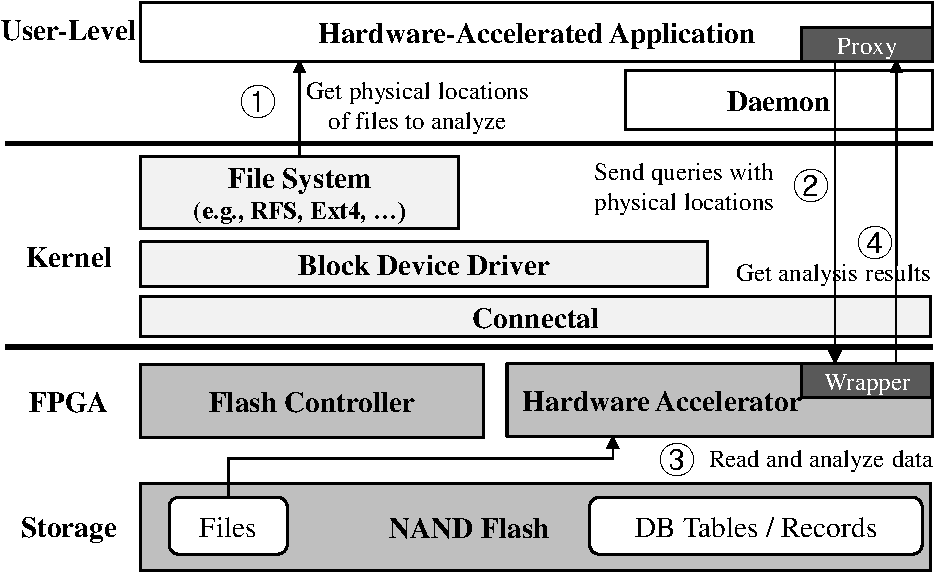
\includegraphics[width=0.4\paperwidth]{figures/software.pdf}
	\caption{Software Interface}
	\label{fig:filesystem}
	\end{center}
\end{figure}
